\newpage
\section{Reconocimiento de expresiones matemáticas}

El problema de reconocer expresiones matemáticas en imágenes consiste en encontrar una función capaz de convertir una imagen preprocesada en una secuencia de caracteres que describa en su totalidad la expresión incluida en la imagen. La imagen de entrada $x$ es preprocesada para obtener una imagen en escala de grises de tal forma que $x \in \mathbb{R} ^ {H x W x 1}$, siendo $H$ y $W$ la altura y el ancho de la imagen respectivamente. La secuencia de caracteres objetivo $y$ es de la forma $y_{1}, y_{2}, \dots , y_{k}$ siendo $k$ la longitud de la secuencia y $y_{i}$ es un caracter válido de \LaTeX{} para el presente Trabajo Terminal.

Para resolver el problema de reconocer expresiones matemáticas, existen aproximaciones secuenciales o globales. De acuerdo con \cite{superprecision} ambos métodos implementados de una forma convencional presentan las siguientes limitaciones: 1) La difícil segmentación de símbolos, 2) el análisis estructural es comúnmente basado en gramáticas libres de contexto, lo cual requiere un conocimiento previo de las expresiones a reconocer para diseñar una gramática, 3) la complejidad de los algoritmos de parseo se incrementa con el tamaño de la gramática usada.

Recientemente el modelo de \textit{Encoder-Decoder} con un sistema de atención comenzó a cobrar relevancia por presentar excelentes resultados en campos de machine learning como el procesamiento del lenguaje natural, segmentación de imágenes e \textit{Image Captioning}. Esta aproximación es completamente opuesta a las soluciones convencionales debido a que es una solución entrenable \textit{end-to-end}, es decir, el modelo puede entrenarse como un todo y no por separado; su capacidad de predicción depende completamente del conjunto de entrenamiento por lo que para mejorar el modelo solo se necesita incrementar la cantidad de datos disponibles sin hacer cambios a la arquitectura de la red; la segmentación de símbolos puede hacerse automáticamente a través de la atención. Por las razones expuestas, se decidió utilizar este modelo de deep learning en el presente Trabajo Terminal.

\subsection{Modelo}

Como se mencionó anteriormente la arquitectura de la red neuronal es del tipo \textit{Encoder-Decoder}, en la Figura \ref{fig:modelo} se muestra un esquema de la red neuronal implementada. La traducción de imágenes se realiza de la siguiente manera: Primero se extraen las características de la imagen en forma de cuadricula utilizando una red convolucional (CNN), luego se procederá a utilizar una versión de dos dimensiones de los \textit{positional encodings} mostrados en el marco teórico y finalmente se procede a reagrupar las filas de la cuadricula en una sola, esta es la fase de codificación. 

\begin{figure}[H]
    \centering
    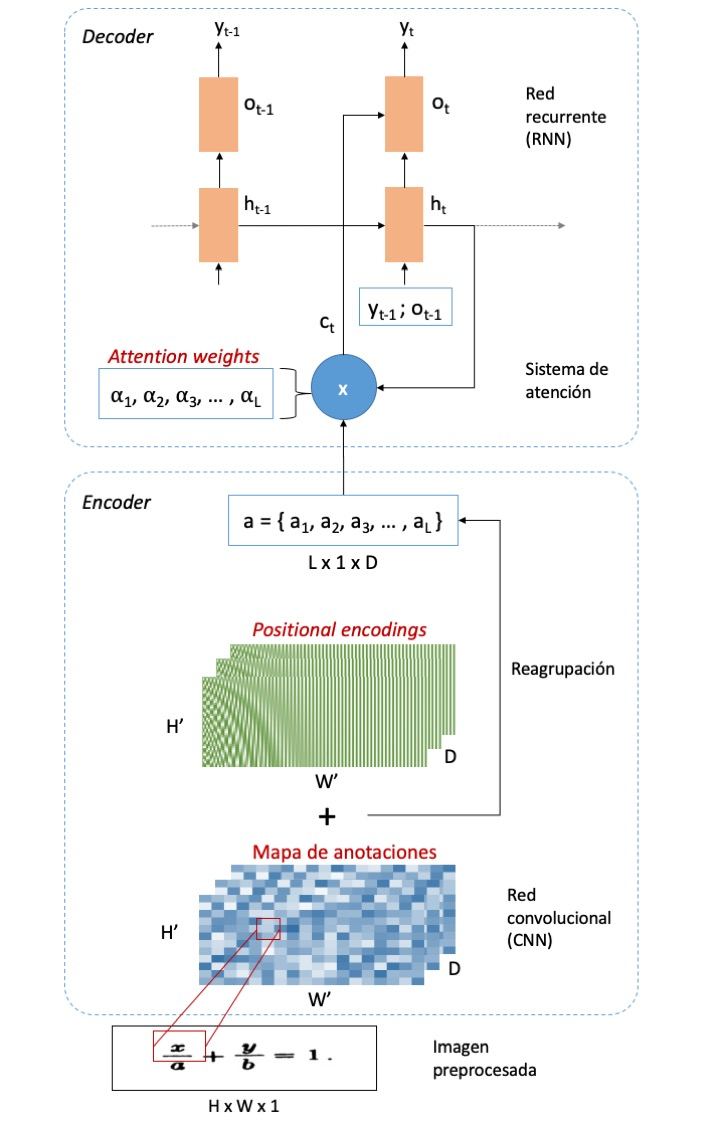
\includegraphics[width=0.8\textwidth]{capitulo5/modelo/img/modelo}
    \caption{Modelo \textit{Encoder-Decoder} de la red neuronal.}
    \label{fig:modelo}
\end{figure}

Para la decodificación, las características codificadas serán usadas por una red neuronal recurrent RNN con un sistema de atención. El \textit{Decoder} implementa un modelo de lenguaje condicional sobre un vocabulario $\lambda$, el cual esta dado por el conjunto de entrenamiento y que será expuesto más adelante.

\subsubsection{Encoder}

La extracción de características de la imagen de entrada $x$ se realiza con una CNN multicapa con \textit{max pooling} y \textit{batch normalization} la cual es ahora un estándar y está completamente inspirada en \cite{harvard}. La Tabla \ref{tbl:cnn-model} resume la arquitectura de la red utilizada. Las características extraídas están almacenadas en vector $v \in \mathbb{R} ^ {H' x W' x D}$, siendo $H'$ y $W'$ las nuevas altura y anchura respectivamente y $D$ el tamaño del último filtro de la red, $D = 512$ en este caso.

\begin{table}[]
\centering
\begin{tabular}{@{}|c|c|c|c|c|c|c|c|@{}}
\toprule
\multirow{2}{*}{Número de capa} & \multicolumn{4}{c|}{Capa Convolucional} & \multicolumn{3}{c|}{Capa de Max Pooling} \\ \cmidrule(l){2-8} 
 & \multicolumn{1}{l|}{Kernel} & \multicolumn{1}{l|}{Strides} & \multicolumn{1}{l|}{Padding} & \multicolumn{1}{l|}{BN} & \multicolumn{1}{l|}{Size} & \multicolumn{1}{l|}{Strides} & \multicolumn{1}{l|}{Padding} \\ \midrule
1 & 64-(3,3) & (1,1) & (1,1) & - & (2,2) & (2,2) & (2,2) \\ \midrule
2 & 128-(3,3) & (1,1) & (1,1) & - & (2,2) & (2,2) & (0,0) \\ \midrule
3 & 256-(3,3) & (1,1) & (1,1) & si & \multicolumn{3}{c|}{-} \\ \midrule
4 & 256-(3,3) & (1,1) & (1,1) & - & (2,1) & (2,1) & (0,0) \\ \midrule
5 & 512-(3,3) & (1,1) & (1,1) & si & (1,2) & (1,2) & (0,0) \\ \midrule
6 & 512-(3,3) & (1,1) & (0,0) & si & \multicolumn{3}{c|}{-} \\ \bottomrule
\end{tabular}
\caption{Especificación de la CNN. El 'Kernel' esta denotado como \textit{número de filtros}-(\textit{dimensiones del filtro}).}
\label{tbl:cnn-model}
\end{table}

Se procede a calcular los \textit{positional encodings}. Existen dos formas de hacer esto, la primera es con parámetros aprendidos y la segunda es con valores fijos. El artículo \cite{harvard} utiliza una RNN bidireccional con el vector $v$ como entrada para aprender estos positional encodings. No obstante, acorde con los inventores de esta técnica \cite{attentionisallyouneed}, los positional encodings fijos producen resultados muy similares a los aprendidos. Así, se optó por utilizar positional encodings fijos y se utlizó la generalización a dos dimensiones propuesta por \cite{positionalencodings}. El vector de positional encodings $pe \in \mathbb{R} ^ {H'xW'xD}$ se obtiene con las siguientes ecuaciones:

\begin{equation}
    pe(w,h,2i) = sin\left(\frac{w}{10000 ^ {\frac{4i}{D}}}\right)
\end{equation}

\begin{equation}
    pe(w,h,2i+1) = cos\left(\frac{w}{10000 ^ {\frac{4i}{D}}}\right)
\end{equation}

\begin{equation}
    pe(w,h,2j+D/2) = sin\left(\frac{h}{10000 ^ {\frac{4j}{D}}}\right)
\end{equation}

\begin{equation}
    pe(w,h,2j+1+D/2) = cos\left(\frac{h}{10000 ^ {\frac{4j}{D}}}\right)
\end{equation}

Con esto, se puede obtener el vector de anotaciones $a$ como sigue:

\begin{equation}
    a = v + pe
\end{equation}

Por último, se reagrupa el vector de anotaciones $a$ de tal forma que $a \in \mathbb{R} ^ {LxD}$, donde $L = H' x W'$, así el vector final de salida del \textit{Encoder} es $a = \{ a_{1}, a_{2}, \dots , a_{L} \}$ con $a_{i} \in \mathbb{R} ^ {D}$.

\subsubsection{Decoder}

Las secuencias $y_{t}$ se generan a partir de un modelo de lenguaje condicional que utiliza las anotaciones $a$ obtenidas en el Encoder. La salida del decoder es la probabilidad de obtener el siguiente token dada la historia de tokens previamente generados y el vector de contexto obtenido mediante la atención.

El modelo de lenguaje condicional es como sigue:

\begin{equation}
    p(y_{t}|y_{1}, \dots , y_{t-1}, a) = softmax(W ^ {out}o_{t})
\end{equation}

con

\begin{equation}
    o_{t} = tanh(W ^ {c}[h_{t}; c_{t}])
\end{equation}

\begin{equation}
    h_{t} = LSTM(h_{t-1}, [y'_{t-1}; o_{t-1}])
\end{equation}

\begin{equation}
    y'_{t} = E y_{t-1}
\end{equation}

donde $W ^ {out}$, $W ^ {c}$ y $E$ son parámetros que serán aprendidos. La matríz $E$, es también conocida en la literatura como la matríz de \textit{embeddings}. El vector $h_{t}$ es utilizado para resumir toda la historia de decodificación y el vector de contexto $c_{t}$ es usado para capturar la información de contexto de la cuadricula de características de la imagen $x$. Los corchetes [;], indican una concatenación entre los vectores dentro de ellos.

Para los estados iniciales $h_{0}$ y $o_{0}$ se utilizó un perceptrón multicapa (MLP) que aprendiera los mejores valores iniciales. Las ecuaciones que describen $h_{0}$ y $o_{0}$ respectivamente son:

\begin{equation}
    h_{0} = tanh(W_{h_{0}}a + b_{h_{0}})
\end{equation}

\begin{equation}
    o_{0} = tanh(W_{o_{0}}a + b_{o_{0}})
\end{equation}

En cada instante $t$, el vector de contexto es calculado. Dado que la mayoría de anotaciones $a$ no contienen información útil para decidir el mejor candidato $y_{t}$, el modelo debe de saber cuáles anotaciones atender. Esta tarea, es delegada a un sistema de atención como el propuesto por \cite{bahdanau2014neural}:

\begin{equation}
    e_{t} = u(h_{t}, a)
\end{equation}

\begin{equation}
    \alpha_{t} = softmax(e_{t})
\end{equation}

\begin{equation}
    c_{t} = \phi(\alpha_{t}, a)
\end{equation}

$\phi$ y $u$ son funciones que pueden ser escogidas libremente, en este caso se utilzarón las mismas que en \cite{harvard}:

\begin{equation}
    e_{it} = \beta ^ {T} tanh(W_{h}h_{i-1} + W_{v}a)
    \label{eq:e-attention}
\end{equation}

\begin{equation}
    c_{t} = \sum_{i} ^ {L} \alpha_{it}a_{i}
\end{equation}

donde $W_{h}$ y $W_{v}$ son parámetros que serán aprendidos. Con esto el modelo de atención puede saber que parte de las anotaciones es importante en el instante $t$. Una consecuencia de esto, es que la segmentación de símbolos es delegada también a este sistema.

Finalmente, se decidió modificar la atención para implementar la técnica del \textit{Coverage Vector} como en \cite{chino}. El coverage vector $F$ se incorporó para dar más información al sistema de atención sobre el historial de la misma atentción, de este modo, es posible mejorar la cobertura global del sistema lo cual ayuda a reducir los errores de símbolos no \texttt{parseados}. El vector de coverage se calcula como sigue:

\begin{equation}
    \eta_{t} = \sum_{l}^{t-1} \alpha_{l}
\end{equation}

\begin{equation}
    F = Q * \eta_{t}
    \label{eq:coverage-vector}
\end{equation}

Donde $\eta_{t}$ es la suma de todos los pesos de las attenciones pasadas y $Q$ es una matriz de pesos que serán aprendidos. De este modo, la Ecuación \ref{eq:e-attention} se modifica por:

\begin{equation}
    e_{it} = \beta ^ {T} tanh(W_{h}h_{i-1} + W_{v}a + W_{f}F)
\end{equation}

de donde $W_{f}$ es una matriz de pesos que serán aprendidos.

\subsection{Implementación}

El lenguaje de programación utilizado para desarrollar la red fue Python 3 junto con el framework para Deep Learning TensorFlow 2. Las unidades usadas en el estado $h_{t}$ de la LSTM son $512$ y $128$ para la dimensión de \textit{embeddings}. El algoritmo de optimización utilizado fue Adam con la Crosentropia Categórica como función de pérdida. 

El código que implementa la red es el siguiente:

\lstinputlisting[language=Python]{capitulo5/modelo/src/encoder.py}

\lstinputlisting[language=Python]{capitulo5/modelo/src/decoder.py}

\subsection{Entrenamiento}

La red fue entranada en el entorno Colaboratory de Google utilizando una GPU, se utilizaron dos conjuntos de entrenamiento. El primero fue CROHME únicamente, mientras que el segundo, fue una combinación entre CROHME y Harvard 100k, esto con la intención de provar cual sería el resultado del modelo si se incrementara el tamaño del conjunto de entrenamiento. Dado que el modelo esta basado solamente en los datos, no fue necesario hacer ningún cambio a la arquitectura.

Para el primer conjunto de entrenamiento, se necesitaron 16 épocas tomando un total de 10 horas. Con respecto al segundo, se entreno la red por 6 épocas tomando un total de 30 horas.

Al utilizar Tensorflow 2, el cálculo de los gradientes de la función de perdida se puede automatizar, así como la actualización de los pesos, no obstante, dada la arquitectura de la red, no es posible utilizar los métodos \textit{compile} y \textit{fit} implementados en Keras para Tensorflow 2. Por lo tanto, el ciclo de entrenamiento tuvo que ser diseñado acorde con las necesidades de la arquitectura propuesta.

El código del ciclo de entrenamiento es el siguiente:

\lstinputlisting[language=Python]{capitulo5/modelo/src/training.py}

\subsection{Resultados}

\subsubsection{Métricas}

Debido a que la arquitectura presentada es un modelo de lenguaje condicional, no sería correcto medir su desempeño solamente evaluando su porcentaje de aciertos totales absolutos contra un conjunto de entrenamiento de prueba. Por esta razón, se utilizaron dos métricas reconocidas en la evaluación de lenguajes condicionales: \textit{BLEU} y \textit{WER}.

La métrica BLEU (Bilingual Evaluation Understudy) es un puntaje utilizado para comparar una traducción candidata contra una o más traducciones referencia. A pesar de ser diseñada para evaluar sistemas de traducción, esta métrica puede ser empleada para evaluar texto generado para una gran variedad de tareas de NLP (Natural Lenguage Processing) entre las que se encuentran el Image Captioning. 

BLEU calcula la precisión $P$ de ngramas o tokens entre dos frases, una candidata y una referencia de la siguiente manera:

\begin{equation}
    P = \frac{ngramas comunes}{ngramas candidata}
\end{equation}

\vspace{1em}

De este modo, tiene en cuenta el número de tokens que fueron correctos. No obstante esto no es suficiente. BLEU penaliza la diferencia de longitudes entre las dos frases:

\begin{equation}
    PB = \left\{ \begin{array}{lcc}
        1 &   si  & c > r \\
        \\ e ^ {1-\frac{r}{c}} &  si & c \leq r \\
        \end{array}
    \right.
\end{equation}

Para calcular BLEU, se utiliza la media geométrica para los $N$ ngramas a utilizar. Cada ngrama tiene un peso $w_{n}$ tal que $\sum_{n = 1}^{N} w_{n} = 1$ con $w_{n} = \frac{1}{N}$ para el presente Trabajo Terminal. Finalmente el puntaje BLEU se obtiene como sigue:

\begin{equation}
    BLEU = PB \exp \left(\sum_{n = 1}^{N}w_{n} \log P_{n} \right)
\end{equation}

\vspace{1em}

Para su implementación, se utilzó la librería NLTK (Natural Lenguage Processing Tool Kit) de Python la cual provee una función para calcular BLEU.

La métrica WER (Word Error Rate) fue derivada de la \textit{distancia de Levenshtein}, la cual es usada en la Teoría de la Información para calcular la diferencia entre dos secuencias. WER, toma en cuenta las sustituciones, inserciones y omisiones que puedan llegar a producirse en las predicciones del modelo, por lo tanto, se dice que WER evalua al modelo a nivel de palabra. 

El puntaje WER, se calcula como sigue:

\begin{equation}
    WER = \frac{S + I + O}{N} = \frac{S + O + I}{S + O + C}
\end{equation}

de donde:

\begin{itemize}
    \item $S$ es el número de sustituciones
    \item $I$ es el número de inserciones
    \item $O$ es el número de omisiones
    \item $N$ es el número de tokens en la referencia
    \item $C$ es el número de tokens correctos
\end{itemize}

Para su implementación se utilizó el código creado por \cite{wer-implementation}.

\subsubsection{CROHME}

Para el caso de la red entrenada con CROHME, se utilizó un conjunto de prueba con 1501 imágenes provistas por CROHME. El \textbf{puntaje BLEU obtenido fue 0.39} y el \textbf{puntaje WER obtenido fue 1.2}. Es decir, la red tiene una precisión de alrededor del $39\%$ para predecir los tokens de una imagen, sin embargo, el puntaje WER al ser muy alto, indica que las predicciones no son confiables y por lo tanto, el modelo no está listo para ser usado en producción. Acorde con \cite{chino}, ellos obtuvieron una precisión del $46.55\%$ sobre CROHME. No obstante, utilizaron los archivos InkML para obtener más información respecto a la trayectoria de las imágenes, brindandoles imágenes de 9 canales, mientras que en el presente trabajo, solo se utilizaron imágenes de 1 canal, por lo que no hay una comparación directa entre los dos trabajos y solo se menciona a modo de referencia.

Con respecto al sistema de atención de este modelo, se puede notar que aún no funciona completamente, esto es debido posiblemente a que la red aún no ha sido capaz de abstraer todas las caracterísitcas importantes del conjunto de entrenamiento. En la Figura \ref{fig:modelo-crohme-loss}, se puede apreciar que a pesar del entrenamiento, la función de pérdida sigue siendo mayor a 5.

\begin{figure}[H]
    \centering
    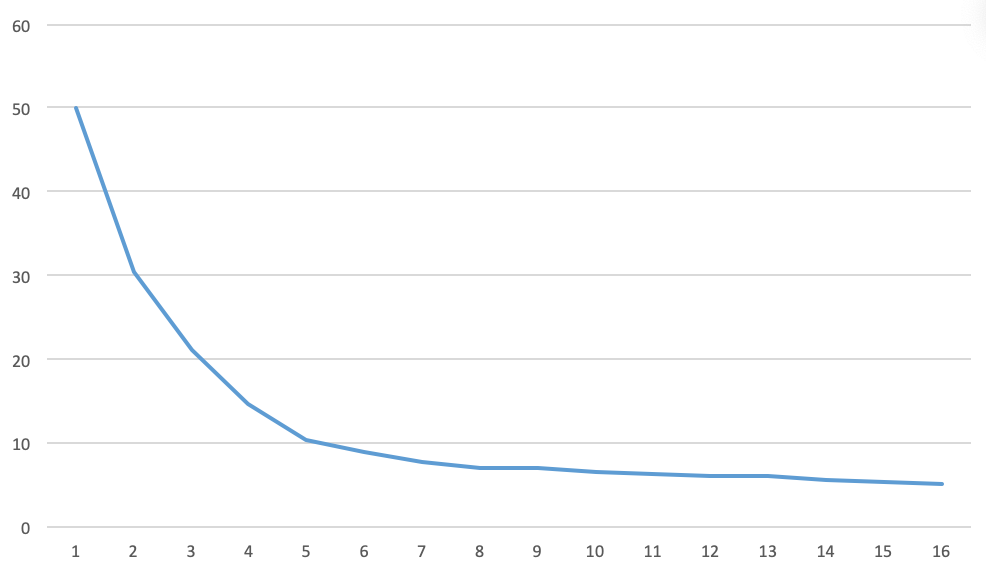
\includegraphics[width=0.5\textwidth]{capitulo5/modelo/img/modelo-crohme-loss}
    \caption{Función de pérdida del modelo entrenado con CROHME.}
    \label{fig:modelo-crohme-loss}
\end{figure}

La razón del pobre desempeño del modelo al momento de generalizar, es el reducido tamaño de CROHME, pues 7169 imágenes no han sido suficientes para obtener un buen resultado en la predicción de expresiones matemáticas escritas a mano. Incrementar la capacidad de la red mediante el aumento del número de parámetros no es una opción viable, pues al ser un conjunto pequeño, el riesgo de sobreentrenamiento auménta considerablemente.

No obstante, se puede observar que la red si ha aprendido a segmentar símbolos y lo que es mucho más sobresaliente, el modelo es capaz de representar las relaciones espaciales y de jerarquía que existen en una expresión matemática, sin embargo, solo es capaz de hacer esto para secuencias cortas. La Figura \ref{fig:modelo-crohme-attention} muestra la comparación de la atención entre dos imágenes, la primera (a), es una secuencia corta mientras que la segunda (b) es una secuencia más larga. 

\begin{figure}[H]
    \centering
    \subfigure[$ \backslash sqrt \{ 2 \} = \backslash frac \{ r \} \{ q \}$]{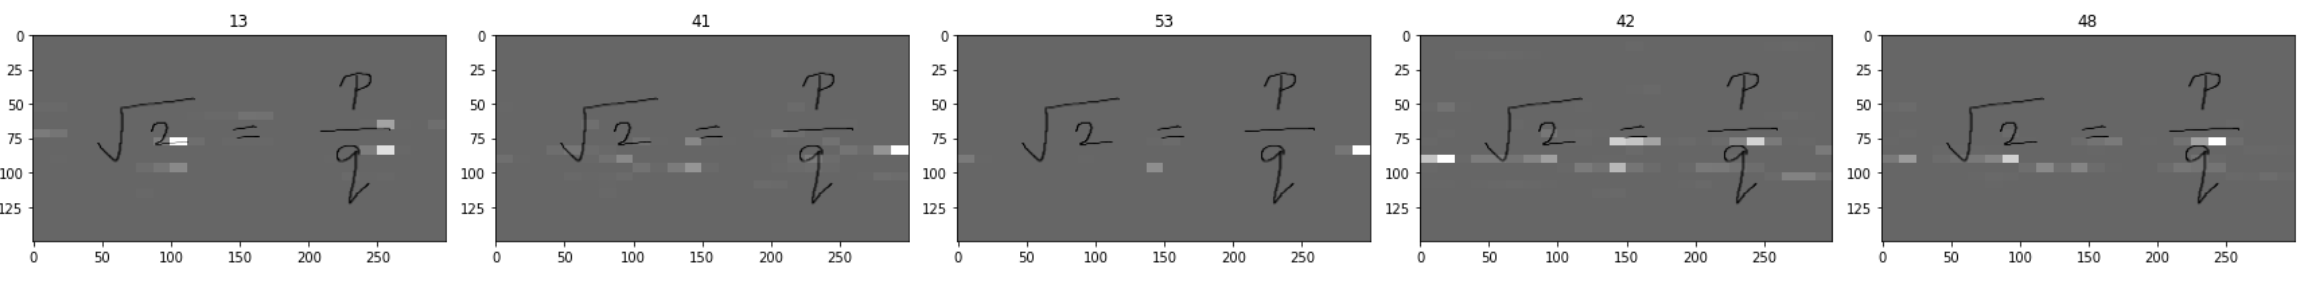
\includegraphics[width=0.9\textwidth]{capitulo5/modelo/img/modelo-crohme-attention1}}
    \subfigure[$ \backslash lim \_ \{ t \backslash rightarrow 0 \} \backslash frac \{ \backslash sin ( x + t ) \} \{ x + 1 \} $]{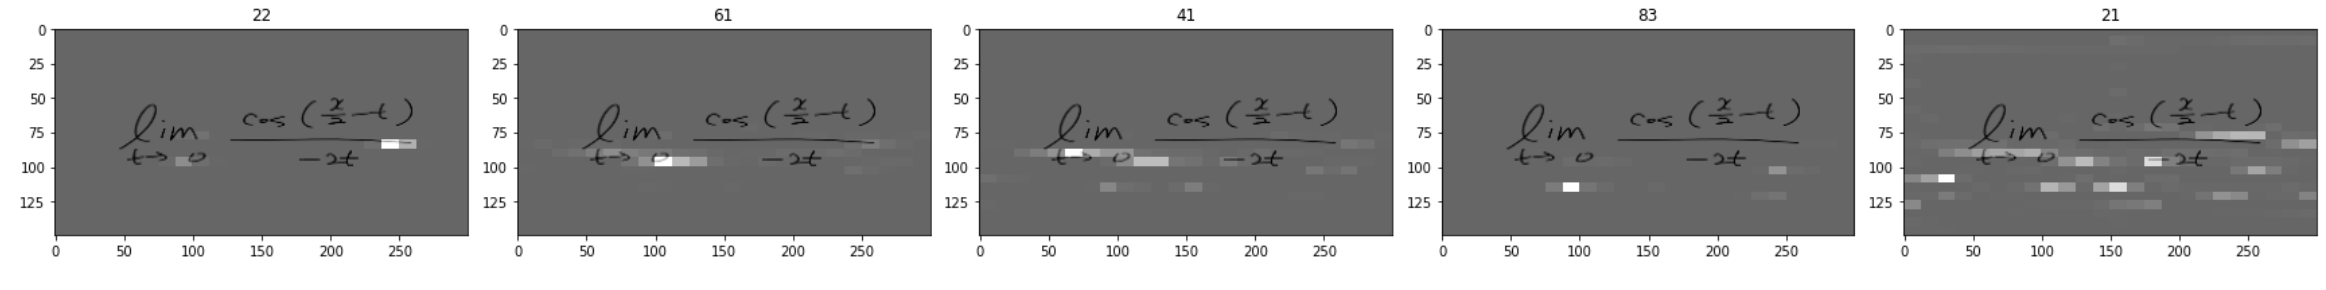
\includegraphics[width=0.9\textwidth]{capitulo5/modelo/img/modelo-crohme-attention2}}
    \caption{(a) Atención de una secuencia corta junto con la secuencia predicha por el modelo. (b) Atención en una secuencia larga junto con la secuencia predicha por el modelo.}
    \label{fig:modelo-crohme-attention}
\end{figure} 

\subsubsection{Harvard 100k}

Con respecto al modelo entrenado con la combinación entre CROHME y Harvard 100k, se utilizó un conjunto de prueba con $9300$ imágenes provistas por Harvard 100k. El \textbf{puntaje BLEU obtenido fue 0.77} y el \textbf{puntaje WER obtenido fue 0.3}. Los resultados obtenidos son satisfactorios al momento de reconocer expresiones matemáticas renderizadas por computadora, pues la precisión de la red es de alrededor de $77\%$, lo que se corresponde con una buena confianza a nivel de palabra por su bajo puntaje WER. En comparación con \cite{harvard}, obtuvimos los mismos resultados de BLEU, y con respecto a WER ellos no calcularon esa métrica. La Figura \ref{fig:modelo-harvard-attention}  muestra los resultados de una predicción de la red. 

No obstante, \textbf{la red no muestra buenos resultados para predecir imágenes con expresiones escritas a mano}. Esto  debido a la gran diferencia entre ambos conjuntos de entrenamiento, a pesar de haber sido combinados ambos conjuntos, CROHME es demasiado pequeño a comparación de Harvard 100k, por lo que CROHME solo introducía ruido al entrenamiento, por lo que actuaba a modo de regularizador más que como ejemplos de los que la red pudiera aprender. 

\begin{figure}[H]
    \centering
    \subfigure[$ L ~ = ~ \backslash sum \_ \{ i \} \backslash operatorname \{ m a z \} ( 0 , 1 \backslash \; - \backslash  a \_ \{ \nu \} + a \_ \{ , \} ) $]{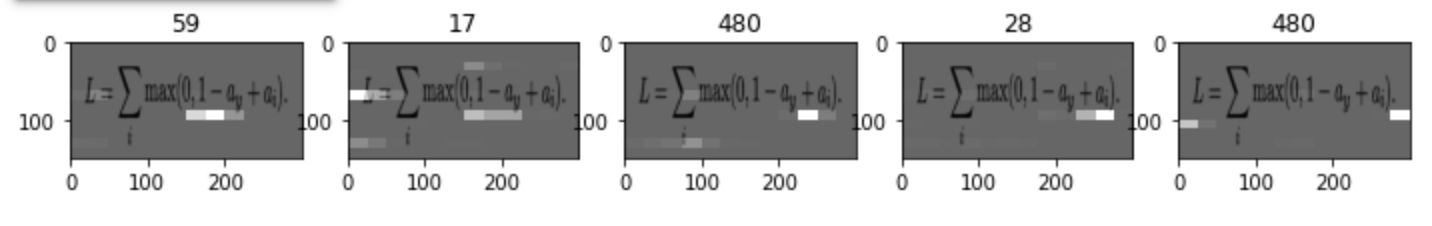
\includegraphics[width=0.9\textwidth]{capitulo5/modelo/img/modelo-harvard-attention}}
    \subfigure[Función de perdida del modelo entrenado con Harvard 100k y CROHME]{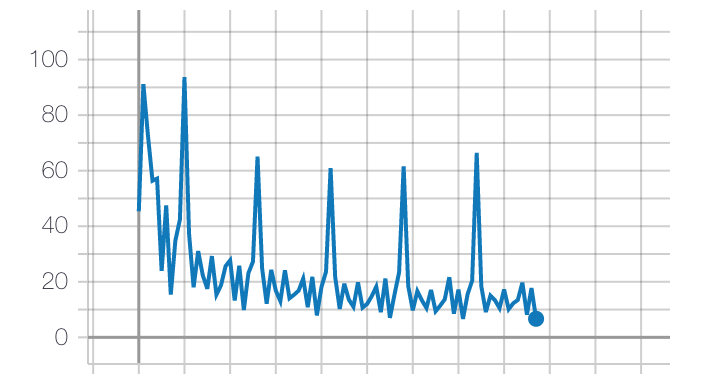
\includegraphics[width=0.5\textwidth]{capitulo5/modelo/img/modelo-harvard-loss}}
    \caption{(a) Atención de una secuencia larga renderizada por computadora junto con la secuencia predicha por el modelo. (b) Función de perdida del modelo.}
    \label{fig:modelo-harvard-attention}
\end{figure}


\subsubsection{Conclusiones}

Comparando los resultados obtenidos de los conjuntos de entrenamiento, se puede ver que el modelo propuesto es capaz de aprender a segmentar símbolos y entender las relaciones bidimensionales que componen a las expresiones matemáticas. No obstante, su efectividad depende completamente del conjunto de entrenamiento, pues este debe de tener un tamaño suficientemente largo y debe de representar adecuadamente las expresiones que se buscan predecir.


\subsection{Experimentos Previos}

Antes de encontrar la configuración adecuada para la red neuronal, se llevaron a cabo varios experimentos. A continuación, se presentan los más relevantes.

\vspace{1em}
\textbf{Variante con GRU}
\vspace{1em}

Se utilizó una GRU como en \cite{gru} en lugar de una LSTM en el \textit{Decoder}. No existe un consenso respecto a cual tipo de RNN basadas en compuertas es mejor, por lo que lo más recomendable es experimentar con ambas. En este caso particular, la GRU no logró abstraer las características del problema. El código fuente del \textit{Decoder} con GRU se muestra a continuación:

\lstinputlisting[language=Python]{capitulo5/modelo/src/gru.py}

Una muestra del resultado del entrenamiento se muestra en la Figura \ref{fig:gru-bad}, en (a) vemos que la función de perdida se estanca, demostrando que no es capaz de modelar el problema en su totalidad mientras que en (b), la atención no mostró aprendizaje alguno.

\begin{figure}[H]
    \centering
    \subfigure[Función de perdida más característica del modelo.]{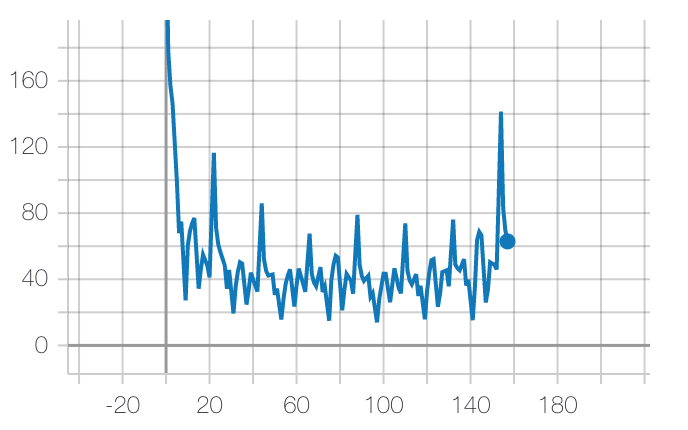
\includegraphics[width=0.5\textwidth]{capitulo5/modelo/img/gru-loss}}
    \subfigure[Atención del sistema.]{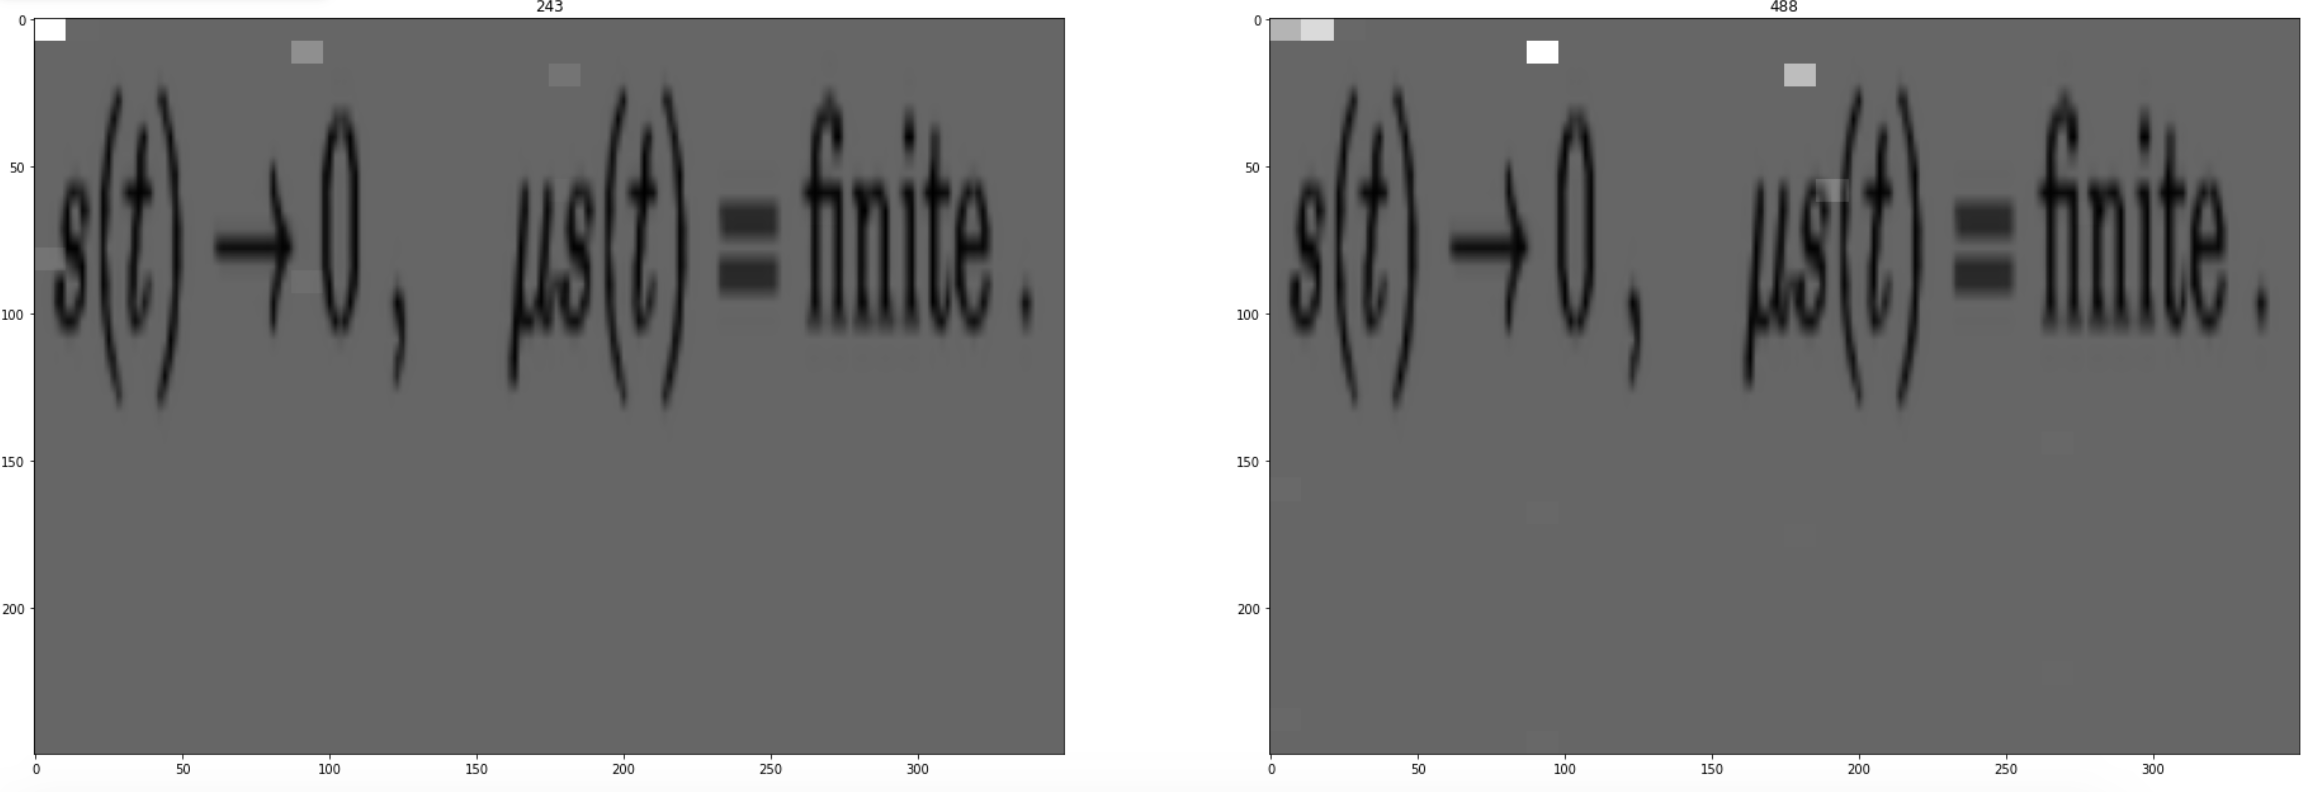
\includegraphics[width=0.5\textwidth]{capitulo5/modelo/img/gru-attention}}
    \caption{(a) Función de perdida del sistema, el modelo se entreno en varias ocasiones, siempre obteniendo una gráfica parecida. (b) Se muestra la atención obtenida por este modelo, se observa un aprendizaje nulo.}
    \label{fig:gru-bad}
\end{figure}


\vspace{1em}
\textbf{Variante con alto Dropout}
\vspace{1em}

Acorde con \cite{deeplearningbook}, el \textit{dropout} es una técnica utilizada para regularizar redes neuronales, es decir, para que la probabilidad de que un modelo se sobreentrene disminuya. Consiste en aplicar un muestreo a las salidas de alguna capa en un modelo con la finalidad de desactivar un porcentaje de neuronas. Suponiendo a $\mu$ como el vector de muestreo y a $p(\mu)$ como la distribución de probabilidad que modela si la neurona se desactiva o no, podemos aplicar dropout a una capa de alguna red neuronal que modele una distribución $p(y|x)$ de la siguiente manera:

\begin{equation}
    P' = p(\mu)p(y|x,\mu)
\end{equation}

De este modo, algunas neuronas \cite{harvard} son "desconectadas" haciendo que cada neurona aprenda sobre la información proveída en el entrenamiento de manera independiente. Esto produce también, un efecto de regularización.

La técnica del dropout es recomendada en la mayoría de los modelos de deep learning, usualmente con una probabilidad de desconexión de $0.5\%$, sin embargo, este radio no provoco ningun efecto en la red. Esto es debido posiblemente a que al ser implementado en las capas convolucionales, un dropout muy alto para una red no tan profunda provoca una perdida significativa de la información. En la Figura \ref{fig:dropout-bad} se pueden ver los resultados de generales de este modelo.

\lstinputlisting[language=Python]{capitulo5/modelo/src/dropout.py}

\begin{figure}[H]
    \centering
    \subfigure[Función de perdida más característica del modelo.]{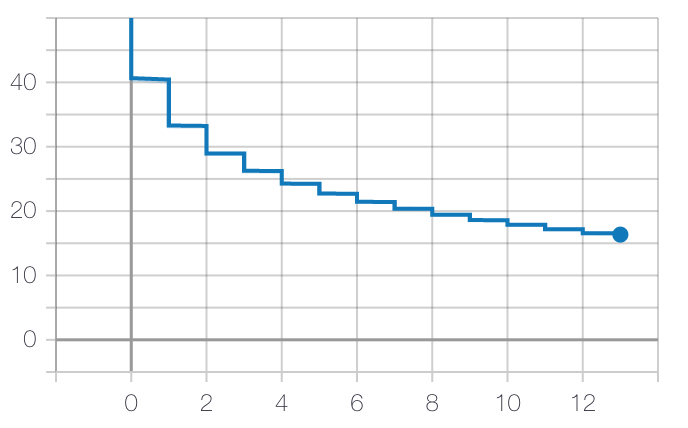
\includegraphics[width=0.5\textwidth]{capitulo5/modelo/img/dropout-loss}}
    \subfigure[Atención del sistema.]{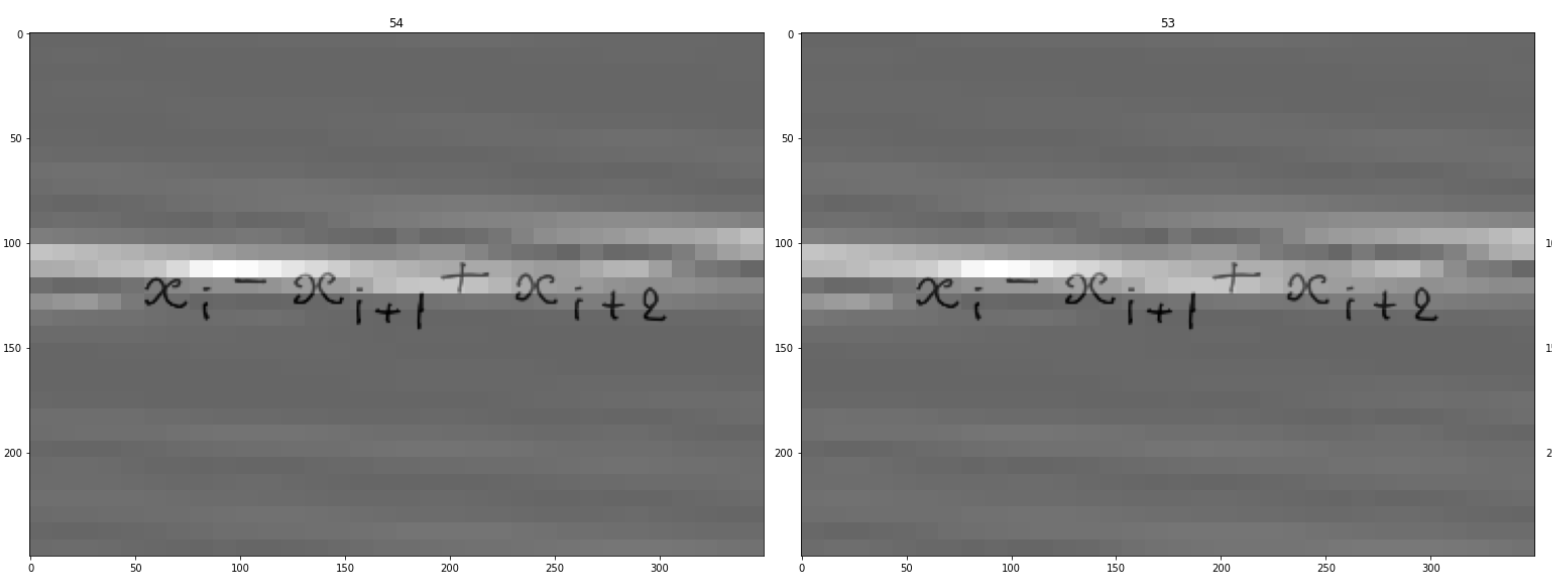
\includegraphics[width=0.5\textwidth]{capitulo5/modelo/img/dropout-attention}}
    \caption{(a) Función de perdida del sistema, el modelo se entreno en varias ocasiones, siempre obteniendo una gráfica parecida. (b) Se muestra la atención obtenida por este modelo, se observa un que el modelo aprendió que a indentificar donde estaba la ecuación, no obstante no aprendio a segmentar los símbolos.}
    \label{fig:dropout-bad}
\end{figure}

 







